\chapter{Ergodic Ensemble Approach to the Material Discovery} \label{chap:crystall}

\section{New Stable Structures?} \label{sec:newstable}

crystALL introduction


\section{Purely data-driven automated structure1
prediction for unidentified chemical compounds} \label{sec:crystall}

A

\begin{figure}[h]
    \centering
    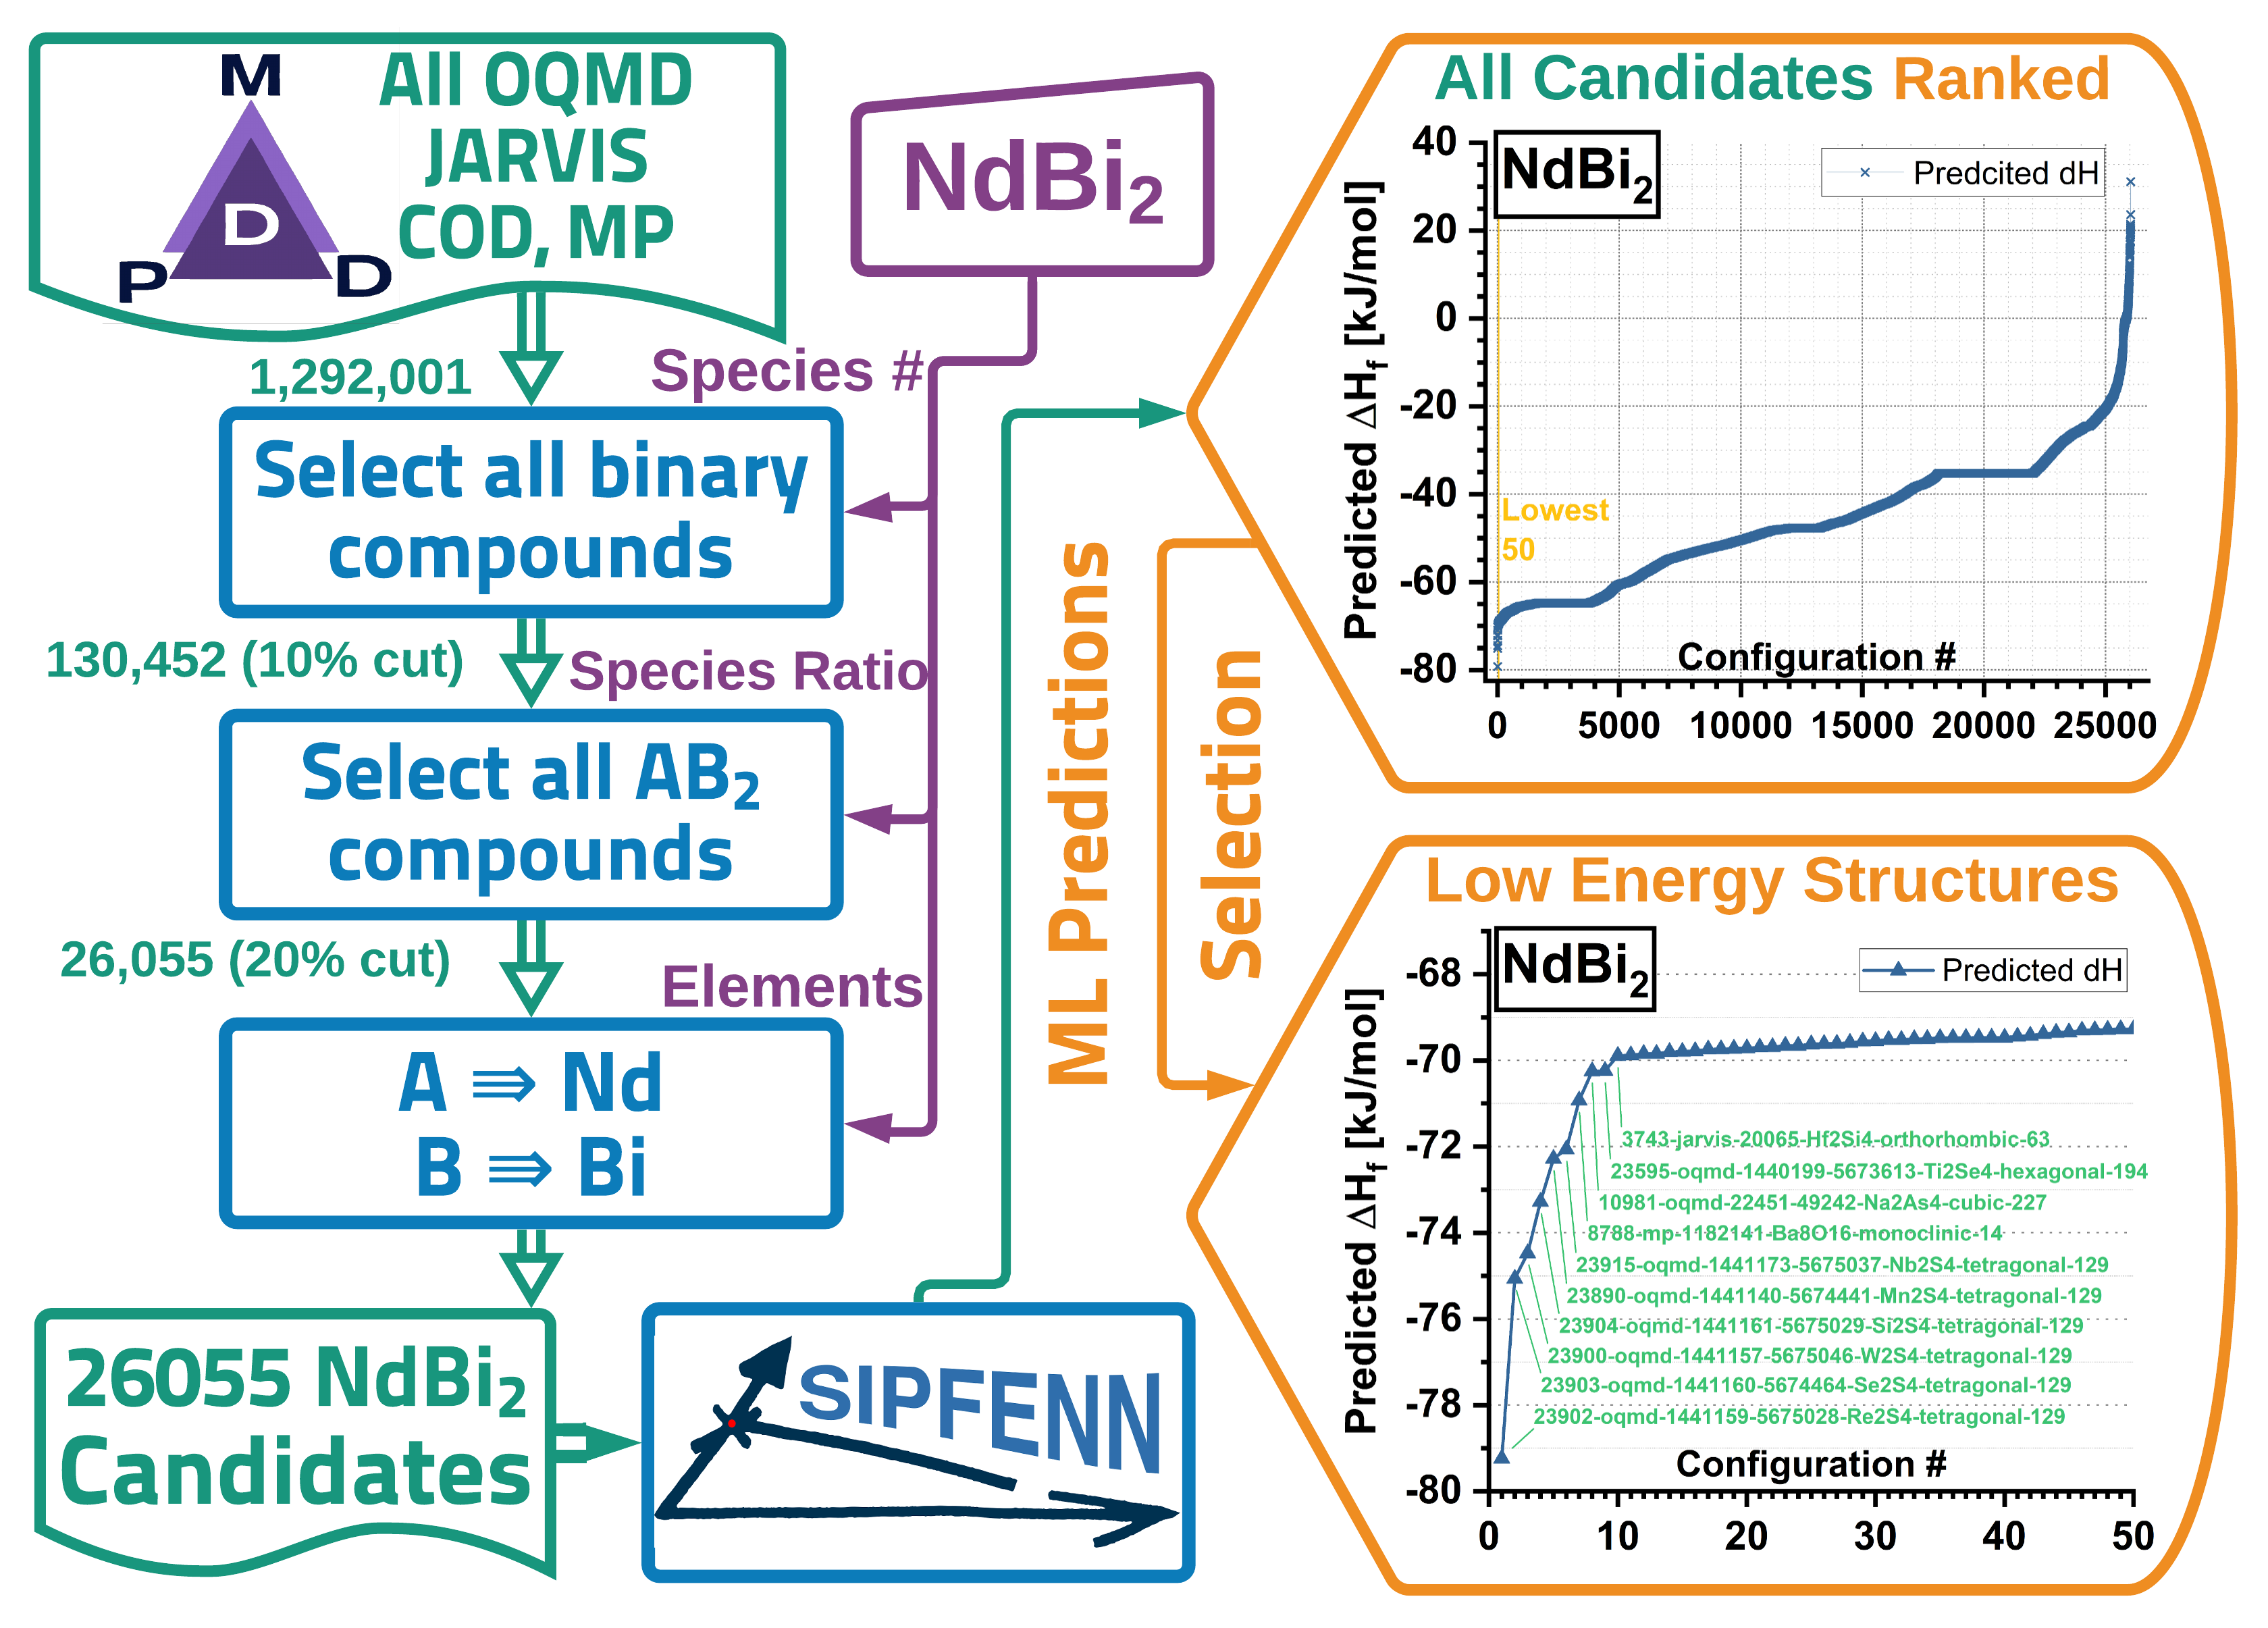
\includegraphics[width=0.9\textwidth]{crystall/NdBi2_GraphicalAbstract_V4.png}
    \caption{\texttt{crystALL} core schematic of operation based around performing all permutations of elemental substitutions and energy predictions, exemplified in the case of $NdBi_2$ intermetallic.}
    \label{fig:crystallcompound}
\end{figure}

\section{Identifying $NdBi_2$ Structure} \se


\section{Predicting Compounds of Uncertain Compositions} \label{sec:crystallcompositional}

B

\begin{figure}[h]
    \centering
    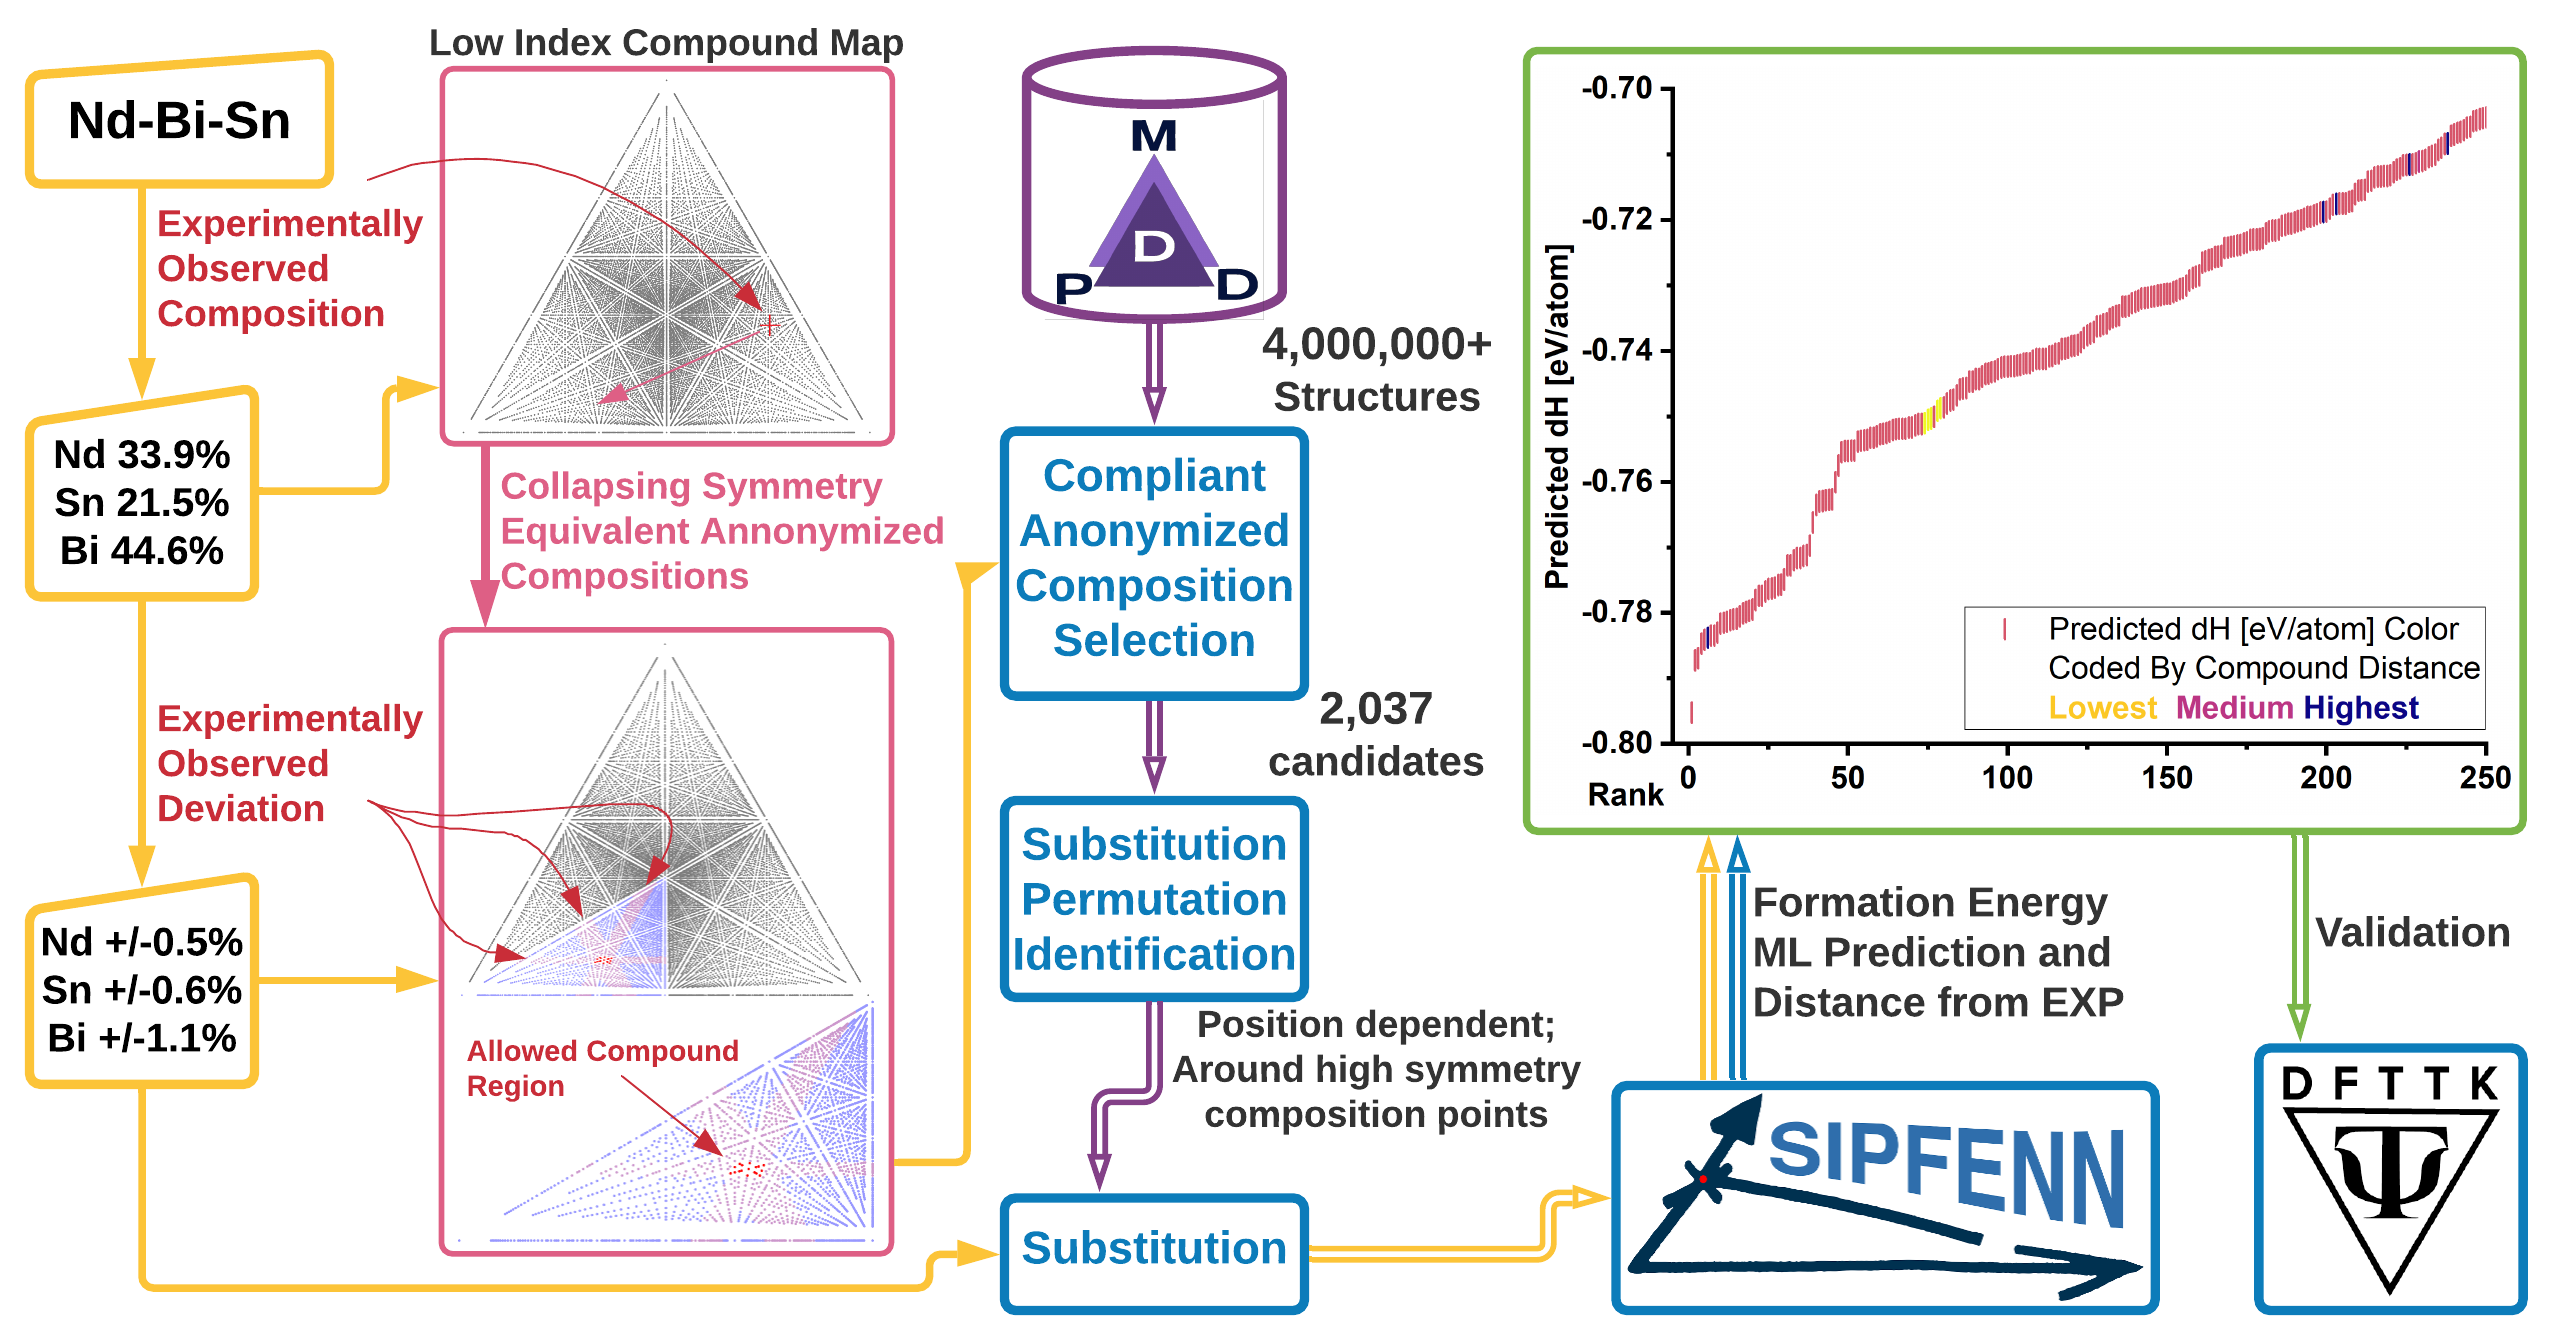
\includegraphics[width=0.9\textwidth]{crystall/crystALL_composition_diagram_V3.png}
    \caption{\texttt{crystALL} schematic of operation in cases of "compositional" searches where measured composition can be given alongside uncertainty bounds. Efficient handling of such queries is a unique feature of MPDD.}
    \label{fig:crystallcomposition}
\end{figure}

\section{Connection to Zentropy} \label{sec:crystallzentropy}

Zentropy


\printbibliography[heading=subbibintoc]